\documentclass[handout]{beamer}
\setbeameroption{show notes}
% March  2013

\usetheme{Berkeley}
\usepackage{amsmath}
\usepackage{array}
\usepackage{graphicx}
\usepackage{graphics}
%\usepackage{pgfpages}
\usepackage{psfrag}
\usepackage{chicago}
\usepackage{todonotes}
\presetkeys{todonotes}{inline}{}
\usepackage{nicefrac}
\usepackage{color}
\usepackage{xcolor}
\usepackage{listings}

%\pgfpagelayout{2 on 1}[a4paper,border shrink=5mm]

\setbeamertemplate{footline}[page number]

\title[User similarity in Twitter]{\bf User similarity in Twitter}
\author[A. Oboturov]{{\bf Artem Oboturov}\\ \texttt{oboturov@telecom-paristech.fr}}
\date{March 22, 2013}

\begin{document}

%%%%%%%%%%%%%%%%%%%%%%%%%%%%%%%%%%%%%%%%%%%%%%%%%%%%%%%%%%%%%%%%%%%%%%%%

\begin{frame}
\titlepage
\end{frame}

%%%%%%%%%%%%%%%%%%%%%%%%%%%%%%%%%%%%%%%%%%%%%%%%%%%%%%%%%%%%%%%%%%%%%%%%

\begin{frame}
\frametitle{\bf Table of Contents}
\tableofcontents
\end{frame}

%%%%%%%%%%%%%%%%%%%%%%%%%%%%%%%%%%%%%%%%%%%%%%%%%%%%%%%%%%%%%%%%%%%%%%%%

\section{Problem statement}

\subsection{What was expected}

%%%%%%%%%%%%%%%%%%%%%%%%%%%%%%%%%%%%%%%%%%%%%%%%%%%%%%%%%%%%%%%%%%%%%%%%

\begin{frame}
\frametitle{\bf What was expected}

\begin{itemize}
\item Similarity network (with Jaccard similarity measure) based on:
\begin{enumerate}
\item keywords
\item items
\item keywords and items together
\end{enumerate}
\item SimRank
\item Data cleaning
\end{itemize}

\end{frame}

%%%%%%%%%%%%%%%%%%%%%%%%%%%%%%%%%%%%%%%%%%%%%%%%%%%%%%%%%%%%%%%%%%%%%%%%

\subsection{Available resources and frameworks}

%%%%%%%%%%%%%%%%%%%%%%%%%%%%%%%%%%%%%%%%%%%%%%%%%%%%%%%%%%%%%%%%%%%%%%%%

\begin{frame}
\frametitle{\bf Available resources and frameworks}

\begin{itemize}
\item Hadoop cluster Mariane @TELECOM ParisTech
\item Hadoop Map Reduce Framework
\item Apache Pig
\end{itemize}

\end{frame}

%%%%%%%%%%%%%%%%%%%%%%%%%%%%%%%%%%%%%%%%%%%%%%%%%%%%%%%%%%%%%%%%%%%%%%%%

\section{Data processing}

\subsection{Pre-Treatement}

%%%%%%%%%%%%%%%%%%%%%%%%%%%%%%%%%%%%%%%%%%%%%%%%%%%%%%%%%%%%%%%%%%%%%%%%

\begin{frame}[fragile]
\frametitle{\bf Dara Pre-Treatement}

\begin{verbatim}
T\t 2009-11-30 23:57:53
U\t http://twitter.com/elissamazing
W\t I just generated a #TweetCloud out of a year of
      my tweets. Top three words: sleep, love, time -
      http://w33.us/476r
\end{verbatim}

Data format:
\begin{description}
\item[T] Time of the tweet
\item[U] Username of the author
\item[W] Tweet content
\end{description}
    
Python script was written to convert it to a (T, U, W) tuple by line file.

\end{frame}

%%%%%%%%%%%%%%%%%%%%%%%%%%%%%%%%%%%%%%%%%%%%%%%%%%%%%%%%%%%%%%%%%%%%%%%%

\subsubsection{Twitter-specific instances}

%%%%%%%%%%%%%%%%%%%%%%%%%%%%%%%%%%%%%%%%%%%%%%%%%%%%%%%%%%%%%%%%%%%%%%%%

\begin{frame}
\frametitle{\bf Twitter-entities extraction}

\begin{description}
\item[Username] extraction and linking matches all valid Twitter usernames but does not verify that the username is a valid Twitter account.
\item[Lists] auto-link and extract list names when they are written in @user/list-name format.
\item[Hashtags] auto-link and extract hashtags, where a hashtag can contain most letters or numbers but cannot be solely numbers and cannot contain punctuation.
\item[URLs]
\end{description}

The \url{https://github.com/twitter/twitter-text-java} Java library was used to perform this step.

\end{frame}

%%%%%%%%%%%%%%%%%%%%%%%%%%%%%%%%%%%%%%%%%%%%%%%%%%%%%%%%%%%%%%%%%%%%%%%%

\subsubsection{Language detection}

%%%%%%%%%%%%%%%%%%%%%%%%%%%%%%%%%%%%%%%%%%%%%%%%%%%%%%%%%%%%%%%%%%%%%%%%

\begin{frame}
\frametitle{\bf Language detection}

The N-Gram model\footnote{"N-Gram-Based Text Categorization" by William B. Cavnar and John M. Trenkle} library\footnote{"Language Detection Library for Java" by S. Nakatani} was used.
It contains an embedded statistical model, i.e. parameters were estimated on a corpora, so no guarantee could be given on text or langauge which would differ in some substantial way.

\end{frame}

%%%%%%%%%%%%%%%%%%%%%%%%%%%%%%%%%%%%%%%%%%%%%%%%%%%%%%%%%%%%%%%%%%%%%%%%

\subsubsection{Stemming}

%%%%%%%%%%%%%%%%%%%%%%%%%%%%%%%%%%%%%%%%%%%%%%%%%%%%%%%%%%%%%%%%%%%%%%%%

\begin{frame}
\frametitle{\bf Stemming}

Phrases normalization was done with the Apache Lucene\footnote{\url{http://lucene.apache.org}}.
Lucene internally uses the Snowball\footnote{\url{http://snowball.tartarus.org}} and the Standard Porter’s stemmer (for English).
Not all languages recognized on the Language detection step are supported by Lucene.
Only those detected and supported by Lucene were considered for further analysis.

\end{frame}

%%%%%%%%%%%%%%%%%%%%%%%%%%%%%%%%%%%%%%%%%%%%%%%%%%%%%%%%%%%%%%%%%%%%%%%%

\subsubsection{URI resolution}

%%%%%%%%%%%%%%%%%%%%%%%%%%%%%%%%%%%%%%%%%%%%%%%%%%%%%%%%%%%%%%%%%%%%%%%%

\begin{frame}
\frametitle{\bf URI resolution}

First, a list of shortener services was created to distinguish between a normal URIs and a shortened ones. The list was compiled from data obtained from following sites:

\begin{itemize}
\item \url{http://code.google.com/p/shortenurl/wiki/URLShorteningServices}
\item \url{http://www.tiny-url.info}
\end{itemize}

In order to resolve URIs a simple crawler could be used which sends HTTP HEAD requests and obtains a Location header value for the 302, 303 and 304 HTTP status codes (redirects).

Resolution time is really slow and idea was abandoned.
\end{frame}

%%%%%%%%%%%%%%%%%%%%%%%%%%%%%%%%%%%%%%%%%%%%%%%%%%%%%%%%%%%%%%%%%%%%%%%%

\subsection{Similarity network construction}

\subsubsection{Hadoop/Pig cross join}

%%%%%%%%%%%%%%%%%%%%%%%%%%%%%%%%%%%%%%%%%%%%%%%%%%%%%%%%%%%%%%%%%%%%%%%%

\begin{frame}[fragile]
\frametitle{\bf Hadoop/Pig cross join}

\lstset{breaklines=true, escapeinside={||}{|>}}
\begin{lstlisting}
tuples_l = LOAD '$INPUT' AS (user_id_l:chararray, values_l:bag {T: tuple(item:chararray)});
tuples_r = LOAD '$INPUT' AS (user_id_r:chararray, values_r:bag {T: tuple(item:chararray)});

||
\textcolor{red}{user\_user\_pairs = CROSS tuples\_l, tuples\_r;}
|>

user_user_pairs_similarity = FOREACH user_user_pairs GENERATE user_id_l, user_id_r, 1.0 - ((double)SIZE(DIFF(values_l, values_r)))/((double)SIZE(BagConcat(values_l, values_r))) AS sim:double;

result_similarity = FILTER user_user_pairs_similarity BY user_id_l != user_id_r AND sim > 0.0;
\end{lstlisting}

\note{
For 390 Mb file after 5 hrs of work consumes of about 35 Gb with temporary data.
Not a feasible solution.
Where this problem comes from?
}

\end{frame}

%%%%%%%%%%%%%%%%%%%%%%%%%%%%%%%%%%%%%%%%%%%%%%%%%%%%%%%%%%%%%%%%%%%%%%%%

\begin{frame}[fragile]
\frametitle{\bf Looking at why it is slow: the Reduce Plan}

\begin{verbatim}
result_similarity: Store(...)
|---Filter[bag]
    |   ... Remove all pairs with zero similarity
    |---user_user_pairs_similarity: New For Each(...)[bag]
        |   Project[chararray][0]
        |   Project[chararray][2]
        |   Subtract[double]
        |   ... Compute value of Jaccard similarity
        |---result_similarity: Filter[bag]
            |   ... Remove reflexive pairs
            |---POJoinPackage(true,true)[tuple]
\end{verbatim}

Join is performed over splits of tuples of this structure:

(\# of Mappers, $1 \leq n \leq $ \# of Mappers, $\ldots$ actual data)

\note{
This is the Reduce Plan for a Cross Join with with supplementary conditions.

Tuples are joined on first field, which is simply a number of Mappers.
}

\end{frame}

%%%%%%%%%%%%%%%%%%%%%%%%%%%%%%%%%%%%%%%%%%%%%%%%%%%%%%%%%%%%%%%%%%%%%%%%

\subsubsection{In-memory cross join}

%%%%%%%%%%%%%%%%%%%%%%%%%%%%%%%%%%%%%%%%%%%%%%%%%%%%%%%%%%%%%%%%%%%%%%%%

\begin{frame}
\frametitle{\bf In-memory cross join}

We can play around caching all data on a processing unit with Large amount of RAM.

\end{frame}

%%%%%%%%%%%%%%%%%%%%%%%%%%%%%%%%%%%%%%%%%%%%%%%%%%%%%%%%%%%%%%%%%%%%%%%%

\section{Implementation iterations}

\subsection{Plain old Java + Hadoop Map-Reduce}

%%%%%%%%%%%%%%%%%%%%%%%%%%%%%%%%%%%%%%%%%%%%%%%%%%%%%%%%%%%%%%%%%%%%%%%%

\begin{frame}
\frametitle{\bf Plain old Java + Hadoop Map-Reduce}

\begin{itemize}
\item Object model required for data representation (Plain old Java)
\item Data serialization (with JSON in our case)
\item Mappers and Reducer are written ad-hoc
\item Input and output are handled manually
\end{itemize}

\end{frame}

%%%%%%%%%%%%%%%%%%%%%%%%%%%%%%%%%%%%%%%%%%%%%%%%%%%%%%%%%%%%%%%%%%%%%%%%

\subsection{Python + Pig UDF + Pig + Java}

%%%%%%%%%%%%%%%%%%%%%%%%%%%%%%%%%%%%%%%%%%%%%%%%%%%%%%%%%%%%%%%%%%%%%%%%

\begin{frame}
\frametitle{\bf Python + Pig + Pig UDF + Java}

\begin{itemize}
\item Python provided simple scripts substituting bash scripts for such task s as data preprocessing and IO
\item Pig was instrumental in working towards goal vs MR whos goal was MR freaking
\item Pig UDF made reuse of existing code from first iteration straight-forward
\end{itemize}

\end{frame}

%%%%%%%%%%%%%%%%%%%%%%%%%%%%%%%%%%%%%%%%%%%%%%%%%%%%%%%%%%%%%%%%%%%%%%%%

\subsection{Scalability on AWS}

\begin{frame}
\frametitle{\bf Scalability on AWS}

To perform data processing on real data set all code was ported to AWS.

\end{frame}

%%%%%%%%%%%%%%%%%%%%%%%%%%%%%%%%%%%%%%%%%%%%%%%%%%%%%%%%%%%%%%%%%%%%%%%%

\section{Conclusion and outlook}

\begin{frame}
\frametitle{\bf Results}

\begin{enumerate}
\item Tweets normalization \textcolor{blue}{was done}
\item Code for similarity network construction \textcolor{blue}{was written and tested on small examples}, for actual data some processing resources are expected to be used
\item For large loads scripts and package \textcolor{blue}{were ported} to the AWS EC2, S3 and EMR
\item SimRank \textcolor{red}{was not implemented}
\end{enumerate}

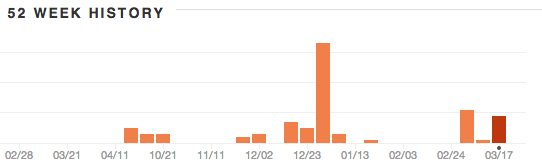
\includegraphics[height=90px]{work-activity.png}

\end{frame}

\end{document}